\documentclass[12pt,a4paper]{article}
\usepackage[margin=1in]{geometry}
\usepackage{parskip}
\usepackage{microtype}
\usepackage{booktabs}
\usepackage{graphicx}
\usepackage{amsmath,amssymb}
\usepackage[most]{tcolorbox}

\title{The period of $\sqrt{n}$\\[0.4em]\large how it was computed, and what distribution $L(n)/\sqrt{n}$ has}
\author{Robin Langer}
\date{}

\begin{document}
\maketitle
\vspace{-1.5em}

This recomputes the histogram in \texttt{\textasciitilde/git/education/fractions/period-histogram.pdf}, whose generating script no longer exists, and then asks the question that figure raises and does not answer.

\section{What was computed}

For every non-square $n$ with $2 \leq n < 10^5$: the period $L(n)$ of the continued fraction of $\sqrt{n}$, and the regulator $R(n)$ of the order $\mathbb{Z}[\sqrt{n}]$.

\begin{center}
\begin{tabular}{lrr}
\toprule
 & September figures & recomputed \\
\midrule
non-squares      & $99{,}683$ & $99{,}683$ \\
shortest period  & $1$        & $1$ \\
longest period   & $750$      & $750$ \\
mean             & $77.84$    & $77.84$ \\
median           & $48$       & $48$ \\
$L > 40$         & $54{,}889$ & $54{,}889$ \\
\bottomrule
\end{tabular}
\end{center}

\section{The algorithm}

The expansion is generated by the PQa recurrence, which holds the surd in exact integer form and never touches a floating point number. Set $a_0 = \lfloor\sqrt{n}\rfloor$, $P_0 = 0$, $Q_0 = 1$, and iterate
\[
  a_i = \left\lfloor \frac{a_0 + P_i}{Q_i} \right\rfloor,
  \qquad
  P_{i+1} = a_i Q_i - P_i,
  \qquad
  Q_{i+1} = \frac{n - P_{i+1}^2}{Q_i}.
\]
The pair $(P_i,Q_i)$ is the state; the complete quotient is $\alpha_i = (P_i + \sqrt{n})/Q_i$.

\textbf{Termination.} The expansion is purely periodic after the first term, and the period closes at the first $i \geq 1$ with $Q_i = 1$. Testing $Q_i = 1$ is preferable to testing $a_i = 2a_0$: the two are equivalent, but the first is an integer comparison against a constant and needs no reference to $a_0$.

Every quantity is an exact integer, so there is no accumulated error and no tolerance to choose. The cost is one division per term, and the total work is $\sum_n L(n) \approx 7.8 \times 10^6$ steps.

\section{The regulator, and one trap}

Over a single period the complete quotients multiply to the fundamental unit of $\mathbb{Z}[\sqrt{n}]$:
\[
  \varepsilon \;=\; \prod_{i=1}^{L} \alpha_i,
  \qquad\text{so}\qquad
  R \;=\; \log\varepsilon \;=\; \sum_{i=1}^{L} \log\alpha_i .
\]
Accumulating logarithms is the only practical route. Forming $\varepsilon = x + y\sqrt{n}$ directly and taking its logarithm overflows a double well before $n = 1000$ --- at $n=61$ the fundamental solution is already $1766319049 + 226153980\sqrt{61}$, and the largest period here is $750$ terms.

\begin{tcolorbox}[colback=yellow!12, colframe=yellow!55!black, arc=2mm]
\textbf{The trap.} The product runs from $i=1$, so each $\alpha_i$ must be read \emph{after} the state has advanced. Reading it before contributes $\alpha_0 = \sqrt{n}$ as a spurious first factor, and every regulator comes out wrong by $\tfrac12\log n$. The first version of this code did exactly that, and the error is invisible without an independent check.
\end{tcolorbox}

\textbf{Validation.} Against three fundamental solutions known in closed form, agreeing to nine decimal places:
\begin{center}
\begin{tabular}{rlrr}
\toprule
$n$ & smallest $x,y$ & $R$ computed & $\log(x+y\sqrt{n})$ \\
\midrule
$2$  & $3,\ 2$                       & $1.762747174$  & $1.762747174$ \\
$13$ & $649,\ 180$                   & $7.168579304$  & $7.168579304$ \\
$61$ & $1766319049,\ 226153980$      & $21.985310765$ & $21.985310765$ \\
\bottomrule
\end{tabular}
\end{center}
When $L$ is odd, $\varepsilon$ has norm $-1$ and the smallest solution of $x^2-ny^2=+1$ is $\varepsilon^2$; the table doubles $R$ in that case. This is the same parity fact that produces the comb.

\section{The comb}

\begin{center}
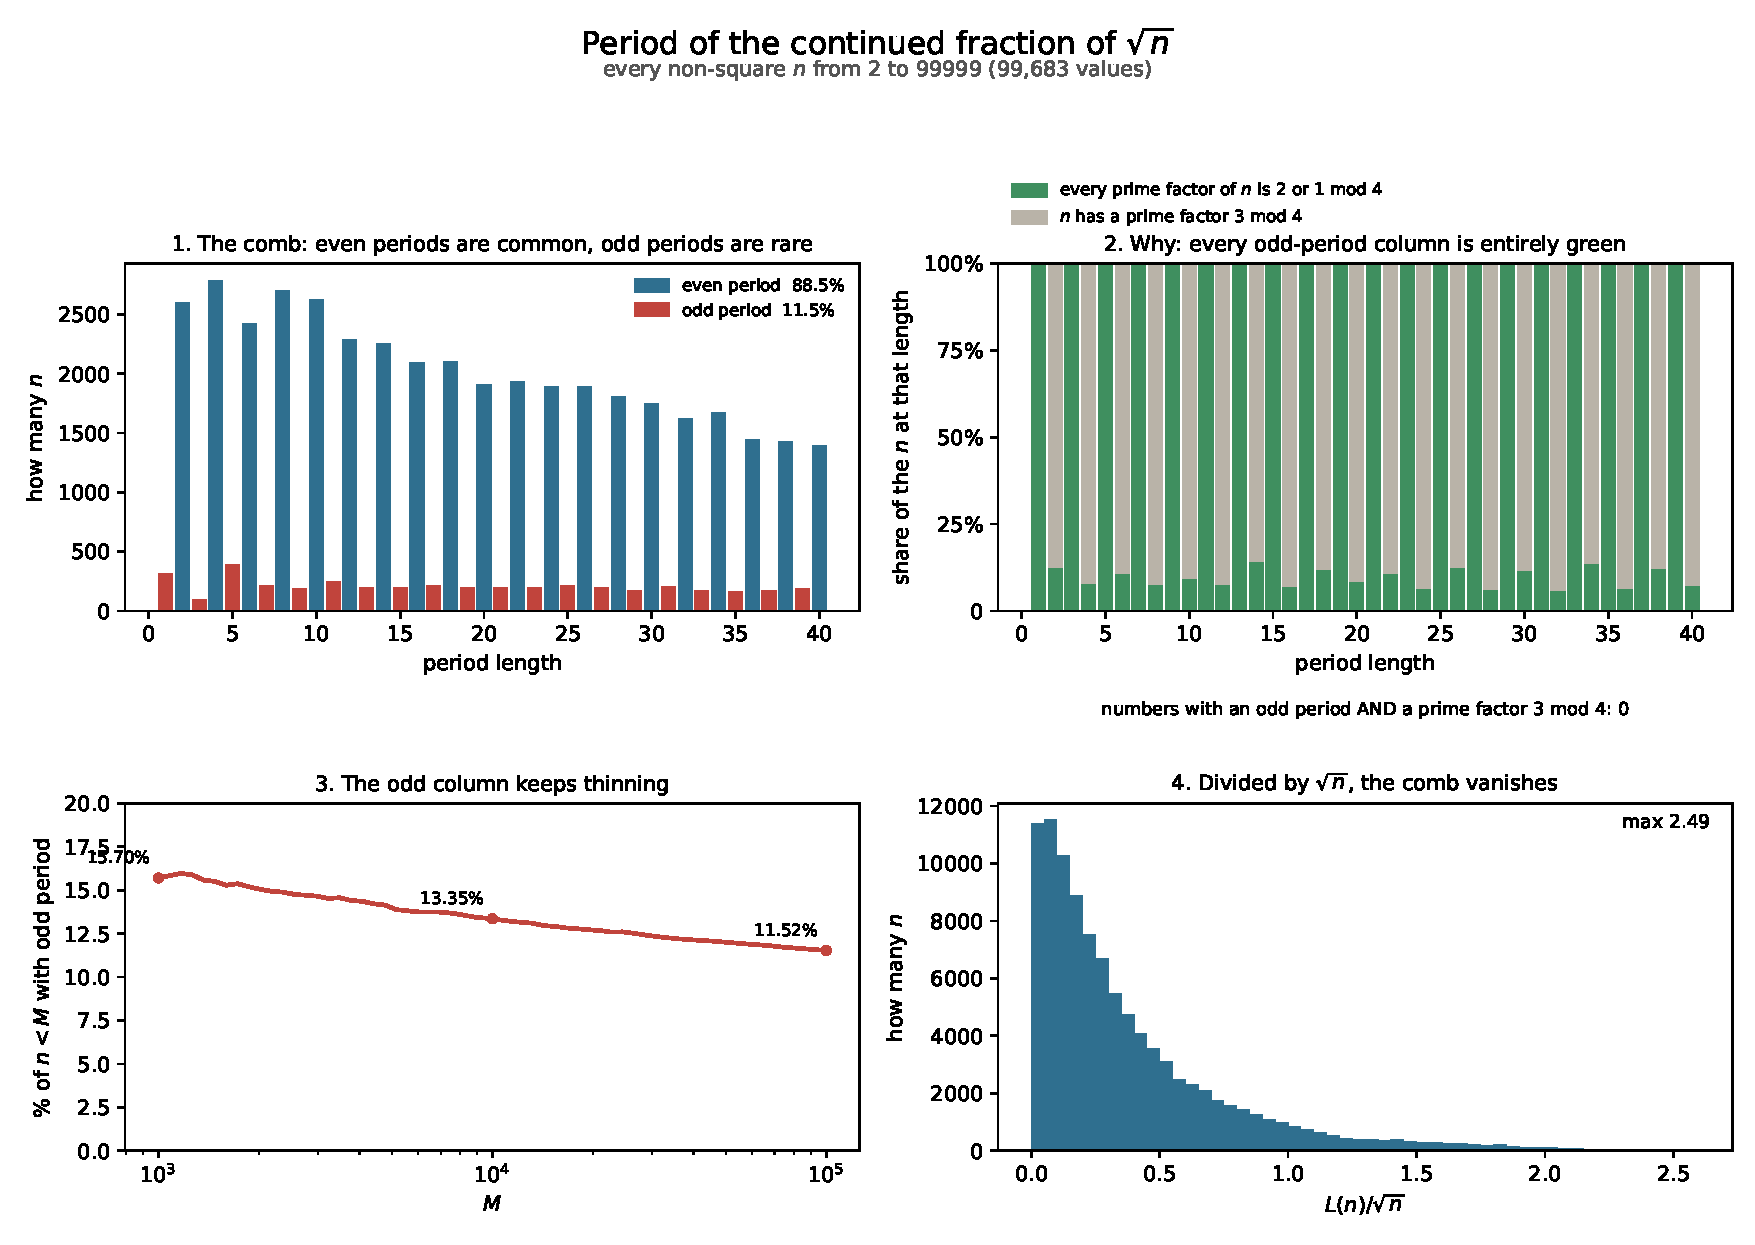
\includegraphics[width=\textwidth]{period-histogram.pdf}
\end{center}

Even periods outnumber odd ones by roughly eight to one, and the ratio worsens with $n$: $15.70\%$ odd below $10^3$, $13.35\%$ below $10^4$, $11.52\%$ below $10^5$.

An odd period means the first pass lands on $-1$, so $x^2-ny^2=-1$ is solvable. If any prime $p \equiv 3 \pmod 4$ divides $n$, reducing that equation mod $p$ gives $x^2 \equiv -1$, making $-1$ a quadratic residue mod $p$ --- impossible for $p \equiv 3 \pmod 4$. So an odd period forces every prime factor of $n$ to be $2$ or $1 \bmod 4$. Roughly three quarters of all integers fail that test, and the proportion creeps up, which is the entire explanation of the comb and of its slow worsening.

The converse is false and is deep: having no prime factor $\equiv 3 \pmod 4$ does not force an odd period. The density of those for which it does is the subject of a conjecture of Stevenhagen.

\section{What distribution is $L(n)/\sqrt{n}$?}

Write $t = L(n)/\sqrt{n}$. The useful move is to split it against the regulator, which is an algebraic identity and free:
\[
  \frac{L(n)}{\sqrt{n}}
  \;=\;
  \underbrace{\frac{L(n)}{R(n)}}_{\text{dynamics}}
  \;\times\;
  \underbrace{\frac{R(n)}{\sqrt{n}}}_{\text{arithmetic}} .
\]

\subsection*{The first factor should be a constant}

$R$ is a sum of $L$ logarithms of complete quotients. If those behave like the complete quotients of a typical continued fraction --- Gauss--Kuzmin --- then their mean logarithm is the L\'evy constant
\[
  \lambda \;=\; \frac{\pi^2}{12\log 2} \;=\; 1.186569,
  \qquad \text{predicting} \qquad
  L/R \to 1/\lambda = 0.842766 .
\]

\begin{center}
\begin{tabular}{lrrr}
\toprule
$n$ range & mean & sd & median \\
\midrule
$[2,10^3)$        & $0.7566$ & $0.2295$ & $0.7817$ \\
$[10^3,10^4)$     & $0.7474$ & $0.1915$ & $0.7944$ \\
$[10^4,5\cdot10^4)$ & $0.7614$ & $0.1679$ & $0.8083$ \\
$[5\cdot10^4,10^5)$ & $0.7705$ & $0.1543$ & $0.8145$ \\
\bottomrule
\end{tabular}
\end{center}

It is drifting upward toward $0.8428$ and the spread is narrowing, but at $10^5$ the median is still $3\%$ short and the relative standard deviation is $21\%$. \emph{So this factor is not yet a constant at this height.} It is consistent with converging to one, and it is not one here.

\subsection*{The second factor carries the arithmetic}

For the real quadratic field of discriminant $D$, the class number formula reads $h\,R \asymp \sqrt{D}\,L(1,\chi_D)$, so
\[
  \frac{R(n)}{\sqrt{n}} \;\asymp\; \frac{L(1,\chi_n)}{h(n)} .
\]
(Stated loosely on purpose: for $n \equiv 1 \bmod 4$ or $n$ non-squarefree, $\mathbb{Z}[\sqrt{n}]$ is not the maximal order and $R$ here is a multiple of the field regulator. That discrepancy is real and is not corrected for anywhere in this document.)

\begin{center}
\begin{tabular}{lrrr}
\toprule
$n$ range & mean & sd & max \\
\midrule
$[2,10^3)$        & $0.6355$ & $0.4035$ & $2.1856$ \\
$[10^3,10^4)$     & $0.5199$ & $0.4361$ & $2.4735$ \\
$[10^4,5\cdot10^4)$ & $0.4637$ & $0.4393$ & $2.8047$ \\
$[5\cdot10^4,10^5)$ & $0.4353$ & $0.4366$ & $2.9049$ \\
\bottomrule
\end{tabular}
\end{center}

The mean falls steadily while the spread stays flat and the maximum climbs. Falling mean with a stable spread is what a growing average class number looks like: more of the $L$-value is being absorbed by $h$ as $n$ grows.

\subsection*{Is it exponential? No, but nearly, in the middle}

A distribution is exponential exactly when its hazard rate $f(t)/P(X>t)$ is constant.

\begin{center}
\begin{tabular}{lrr@{\qquad}lrr}
\toprule
$t$ & count & hazard & $t$ & count & hazard \\
\midrule
$0.00$--$0.13$ & $29{,}207$ & $2.254$ & $0.91$--$1.04$ & $2{,}511$ & $2.072$ \\
$0.13$--$0.26$ & $21{,}788$ & $2.378$ & $1.04$--$1.17$ & $1{,}774$ & $2.003$ \\
$0.26$--$0.39$ & $14{,}624$ & $2.310$ & $1.17$--$1.30$ & $1{,}123$ & $1.715$ \\
$0.39$--$0.52$ & $9{,}786$  & $2.210$ & $1.30$--$1.43$ & $952$     & $1.871$ \\
$0.52$--$0.65$ & $6{,}631$  & $2.101$ & $1.43$--$1.56$ & $811$     & $2.105$ \\
$0.65$--$0.78$ & $4{,}807$  & $2.095$ & $1.56$--$1.69$ & $653$     & $2.334$ \\
$0.78$--$0.91$ & $3{,}517$  & $2.107$ & $1.69$--$1.82$ & $561$     & $2.879$ \\
\bottomrule
\end{tabular}
\end{center}

Across the bulk, $0.4 \lesssim t \lesssim 1.2$, the hazard sits between $2.0$ and $2.3$ --- flat enough that an exponential of rate about $2.1$ is a fair description of the middle of the distribution. It is not flat at either end. It is higher near zero, and from $t \approx 1.4$ it climbs steeply, reaching $2.88$ in the last populated bin. A rising hazard means a tail \emph{lighter} than exponential: having already reached $t$, the variable becomes progressively more likely to stop soon. That is the analytic content of the ``hard looking right hand edge'' --- the edge is real, and it is soft.

\subsection*{The answer}

\begin{tcolorbox}[colback=blue!6, colframe=blue!45!black, arc=2mm]
$L(n)/\sqrt{n}$ is not a standard named distribution, and more importantly it is \textbf{not a fixed distribution at all}. It is approximately exponential with rate $\approx 2.1$ through the bulk, with a lighter-than-exponential tail beyond $t \approx 1.4$, and its shape \emph{drifts with $n$}. Both factors drift, in opposite directions: the dynamical factor $L/R$ rises toward $1/\lambda$, and the arithmetic factor $R/\sqrt{n}$ falls as the average class number grows.
\end{tcolorbox}

\begin{center}
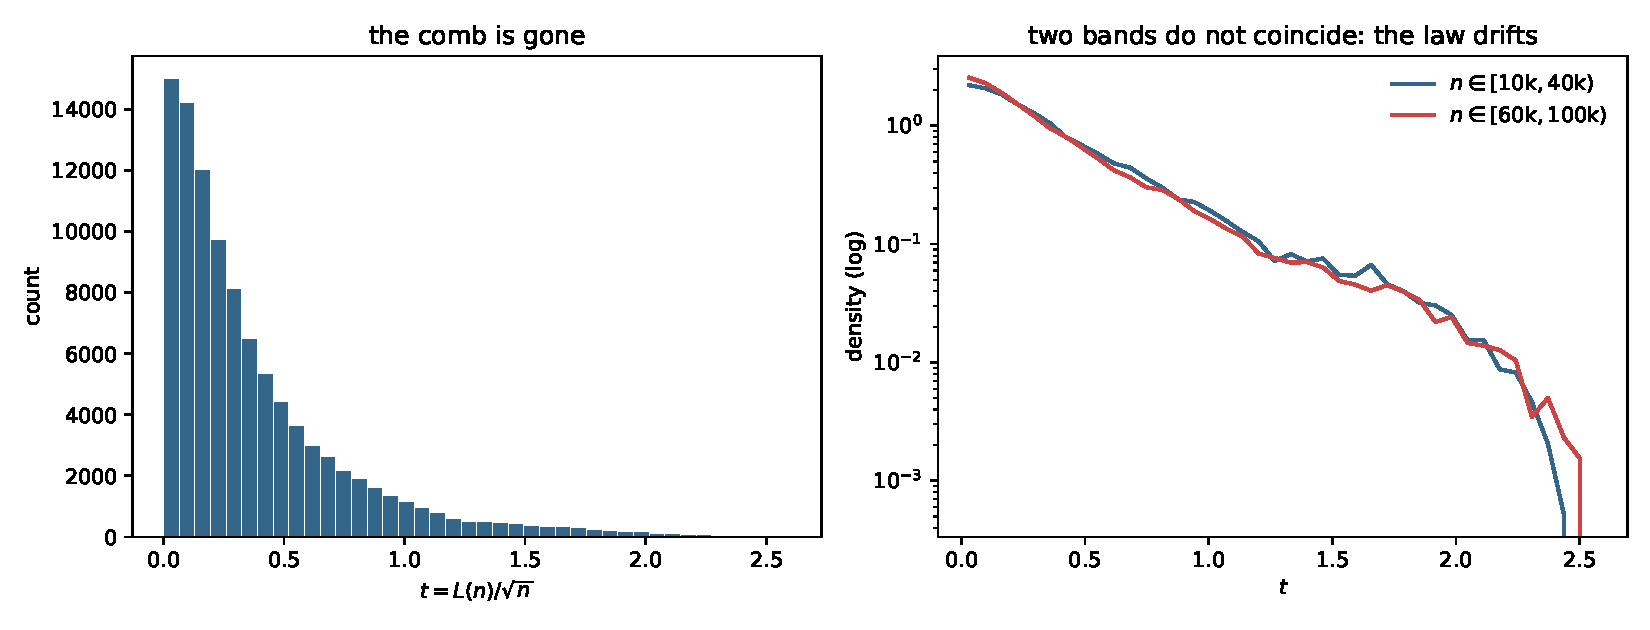
\includegraphics[width=\textwidth]{distribution.pdf}
\end{center}

The right-hand panel plots the density on two disjoint bands. They do not coincide. This is the direct explanation of the negative result in \texttt{learned-curve.pdf}, where a curve fitted on $n \in [300\,000,400\,000)$ transferred badly to $n \in [100\,000,160\,000)$ --- held-out error $0.112$ rising to $0.183$. No fit can transfer, because the target is not the same object in the two bands.

\section{How the mean grows}

\begin{center}
\begin{tabular}{rrrrr}
\toprule
$M$ & mean $L$ & $/\sqrt{M}$ & $\times \log M$ & $\times \sqrt{\log M}$ \\
\midrule
$3{,}000$   & $17.06$ & $0.3116$ & $2.4945$ & $0.8816$ \\
$10{,}000$  & $28.38$ & $0.2838$ & $2.6136$ & $0.8612$ \\
$30{,}000$  & $45.94$ & $0.2653$ & $2.7345$ & $0.8517$ \\
$100{,}000$ & $77.84$ & $0.2462$ & $2.8341$ & $0.8353$ \\
\bottomrule
\end{tabular}
\end{center}

The raw ratio falls about $10\%$ per step, so the growth is not a clean power near $0.44$. Dividing by $\log M$ overshoots (the column rises); dividing by $\sqrt{\log M}$ undershoots (it falls). Fitting $\text{mean}/\sqrt{M} = c\,(\log M)^{-\theta}$ across the four rows gives $\theta \approx 0.65$. The truth is bracketed strictly between $\sqrt{M}/\log M$ and $\sqrt{M}/\sqrt{\log M}$, and $10^5$ is not high enough to separate them.

\section{What would settle it}

\begin{enumerate}
\item \textbf{Run to $10^6$.} Cost is $\sum L(n) \approx 2.5\times 10^8$ steps, which wants the inner loop in C or Rust rather than Python. That separates the two candidate laws for the mean and shows whether $L/R$ has reached $1/\lambda$.
\item \textbf{Compute $h(n)$.} The decomposition above is inferred, not measured: no class number is calculated anywhere here. Computing $h$ on a sample of a few thousand $n$ per band would test directly whether $R\,h/\sqrt{n}$ is the scale-invariant variable, and whether $L(1,\chi)$ is what remains.
\item \textbf{Use the field, not the order.} Restricting to squarefree $n \equiv 2,3 \bmod 4$ removes the maximal-order discrepancy flagged above, at the price of about half the data.
\end{enumerate}

\end{document}
